\chapter{Differential Exposure Estimation}

\section{Single-step Exposure}

The central objective of this project is to estimate whether different controlled user profiles are associated with different patterns of dark pattern exposure during mobile application interaction. To support this objective, the analysis begins at the level of a single interaction step. Each step in the audit corresponds to one observable interface state produced after a profile-conditioned action is executed. In practice, this state is recorded as a screenshot or a comparable interface observation. The screenshot is then manually annotated using the seven-dimensional Dark Pattern Score vector, abbreviated as DPS.

Formally, the exposure observed at interaction step \(t\) is represented as

\[
D_t = [I_t, F_t, P_t, C_t, S_t, N_t, FA_t],
\]

where \(I_t\) denotes Interface Interference, \(F_t\) denotes Friction, \(P_t\) denotes Pressure, \(C_t\) denotes Contextual Deception, \(S_t\) denotes Sneaking, \(N_t\) denotes Nagging, and \(FA_t\) denotes Forced Action. The vector \(D_t\) therefore represents the dark pattern exposure observed in a single interface state at step \(t\). This formulation follows the broader idea in dark pattern research that deceptive or manipulative interface mechanisms can be operationalized into observable categories rather than treated only as anecdotal examples \cite{gray2018darkpatterns,mathur2019darkpatterns,mathur2021whatmakesdark}.

The single-step vector is intentionally simple. It does not attempt to explain why the interface state appeared, nor does it claim that the user profile caused the application to display that state. Instead, it provides a structured measurement of what was observed after a controlled interaction. A raw component \(D_{t,d}\) is a numeric exposure score, and the binary occurrence variable for that component is \(1[D_{t,d}>0]\). This distinction is important because the project is designed as a profile-aware audit of exposure, not as a causal inference study of platform decision-making. A single vector \(D_t\) should therefore be interpreted as one observed unit of exposure within a longer interaction trajectory.

\section{Profile-level Exposure}

While a single screenshot can reveal whether a particular interface state contains dark pattern mechanisms, it is not sufficient for comparing user profiles. Mobile applications are dynamic systems: pop-ups, recommendations, payment prompts, discounts, and consent interfaces may appear at different moments during interaction. For this reason, the project estimates exposure over repeated interaction steps rather than relying on isolated screenshots.

For a given profile \(A\), the profile-level exposure is defined as the empirical mean of all single-step DPS vectors collected under that profile:

\[
E(D \mid A) = \frac{1}{n_A}\sum_{t=1}^{n_A} D_t.
\]

Here, \(n_A\) is the effective number of audited interaction steps available for profile \(A\), and \(D_t\) is the DPS vector observed at step \(t\). In the project design, each profile is assigned the same target budget, but the archived analysis uses the effective observed length because five trajectories end before the 30-step target. Each profile is audited through repeated controlled interactions, and the resulting vectors are averaged to estimate the typical exposure pattern associated with that profile.

Each dimension of \(E(D \mid A)\) represents either a raw intensity mean or a binary occurrence rate, depending on the analysis. For occurrence-rate analysis, each raw score is first converted to \(1[D_{t,d}>0]\), so a Pressure value of \(0.40\) means that pressure-related mechanisms appeared in approximately 40 percent of the audited interaction states for that profile. For intensity analysis, the raw numeric values are averaged directly, so means can exceed 1 for dimensions scored with counts or ordinal levels. This interpretation makes the exposure vector intuitive while preserving the distinction between whether a mechanism appears and how strongly it appears.

The profile-level estimate is especially useful because the project constructs three controlled user profiles: a high-payment shopping profile, a low-payment browsing profile, and a bargain-hunter profile. These profiles differ in their interest distributions and behavior distributions, but they exclude demographic attributes to improve controllability and reproducibility. Therefore, \(E(D \mid A)\) estimates profile-conditioned exposure under controlled behavioral assumptions rather than exposure for real demographic groups.

\section{Application-level Exposure}

The profile-level estimate summarizes exposure across the audit data for a given profile, but it does not show whether profile differences are consistent within the same application. To address this, the framework also defines application-level exposure:

\[
E(D \mid A, app) = \frac{1}{n_{\mathrm{app},A}}\sum_{t=1}^{n_{\mathrm{app},A}} D_{app,A,t}.
\]

In this expression, \(D_{app,A,t}\) denotes the DPS vector observed in application \(app\), under profile \(A\), at interaction step \(t\). The value \(n_{\mathrm{app},A}\) refers to the effective number of archived interaction steps for that profile within that application. This estimate allows the analysis to compare different profiles while holding the application fixed.

Application-level exposure is important because different mobile applications may implement different interface strategies. A shopping application may emphasize discounts, urgency, and recommendation placement, while a food-delivery application may rely more heavily on login gates, membership prompts, or payment-related decision points. By computing \(E(D \mid A, app)\), the framework can ask whether the high-payment profile encounters more pressure-related exposure than the low-payment profile inside the same application, rather than merely across the full dataset.

Application-level heatmaps make it possible to observe whether profile-conditioned exposure differences are concentrated in particular mechanisms, such as Interface Interference or Pressure. The representative heatmaps in Chapter~\ref{chap:results} use this format to compare exposure across profiles and DPS dimensions. However, the interpretation should remain cautious. A higher value for one profile indicates an observed association between the controlled profile and the exposure pattern in the audit setting; it does not prove the internal logic by which the application generated the interface state.

\section{Category-level Exposure}

In addition to analyzing individual applications, the framework aggregates exposure at the application-category level. Category-level exposure is defined as

\[
E(D \mid A, category),
\]

where \(category\) denotes a group of applications sharing a similar service context, such as shopping, food delivery, entertainment, or social content platforms. In practice, this value can be estimated by averaging the application-level exposure vectors for all applications within the same category, under the same profile.

Category-level exposure is useful because dark pattern mechanisms may be shaped by the functional goals of the application category. For instance, food-delivery applications may require users to log in, choose delivery addresses, enable location access, or enter payment-related information before completing core tasks. As a result, this category may show consistently high Forced Action exposure. By contrast, shopping applications may more frequently display pressure-related elements, such as limited-time offers, promotional rankings, or interface emphasis on high-value items. These patterns are not interpreted as universal properties of the categories, but as observed tendencies in the audited sample.

Category-level exposure estimates help reduce the noise of individual applications and make it easier to identify broader exposure patterns. At the same time, category-level results should not hide application-level variation. Two applications in the same category may still differ substantially in their interface design, business model, and personalization mechanisms.

\section{Pairwise Profile Difference}

To directly compare two profiles, the framework defines a pairwise exposure difference vector:

\[
\Delta(A_i, A_j) = E(D \mid A_i) - E(D \mid A_j).
\]

The resulting vector has the same seven dimensions as the DPS vector. Each component indicates whether profile \(A_i\) encountered more or less of a given dark pattern mechanism than profile \(A_j\). For example, if the Pressure component of \(\Delta(A_i, A_j)\) is positive, then profile \(A_i\) showed higher estimated pressure exposure than profile \(A_j\). If the Forced Action component is close to zero, then the two profiles encountered similar levels of forced-action exposure in the audited data.

This difference vector is more informative than a single aggregate score because dark pattern exposure is multidimensional. Two profiles may have similar overall exposure levels but differ in the mechanisms they encounter. For instance, the high-payment shopping profile and the bargain-hunter profile may both show elevated exposure, but the former may be associated with more high-value product steering while the latter may be associated with more discount urgency or promotional pressure. The pairwise vector preserves this dimensional structure and helps identify which specific DPS mechanisms contribute to the observed profile difference.

\section{Overall Distance Between Profiles}

\begin{figure}[htbp]
    \centering
    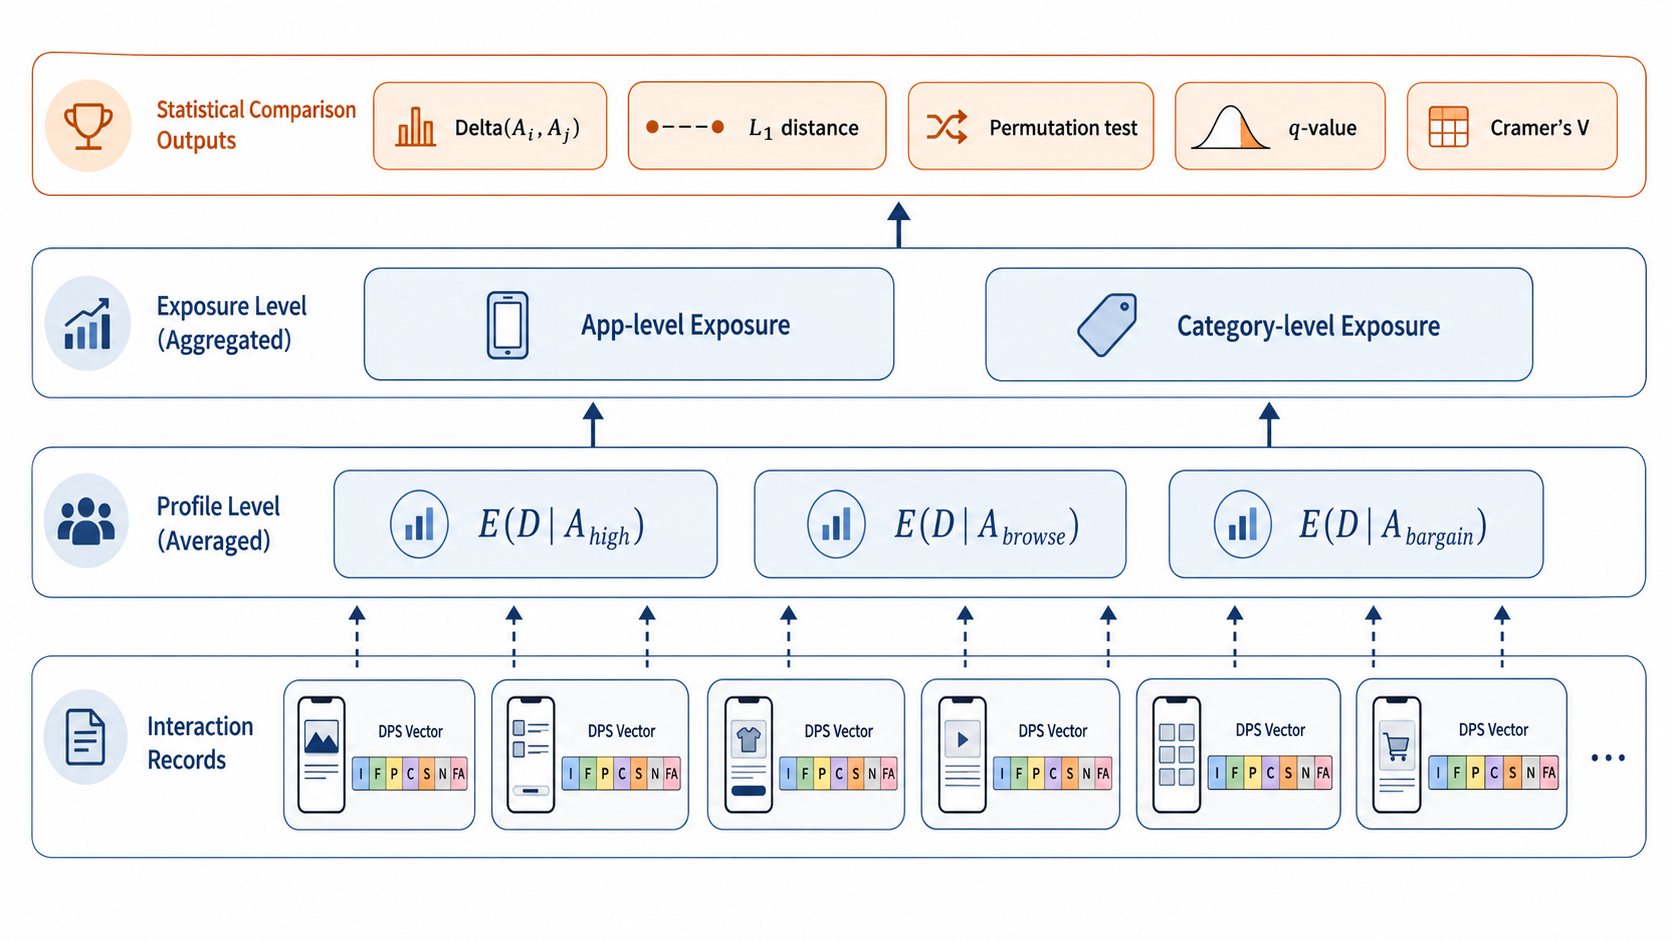
\includegraphics[width=0.95\linewidth]{figures/pictures/exposure_estimation_hierarchy.png}
    \caption{Exposure Estimation Hierarchy}
    \label{fig:exposure-estimation-hierarchy}
\end{figure}

Although the pairwise difference vector is useful for dimension-level interpretation, it is sometimes helpful to summarize the overall magnitude of difference between two profiles. For this purpose, the framework uses the \(L_1\) distance between exposure vectors:

\[
L_1(A_i, A_j) = \sum_{d \in \{I,F,P,C,S,N,FA\}}
\left| E(D_d \mid A_i) - E(D_d \mid A_j) \right|.
\]

Here, \(D_d\) denotes one of the seven DPS dimensions. The \(L_1\) distance sums the absolute exposure differences across all dimensions. A larger value indicates a larger practical difference between the two profile-level exposure patterns, while a smaller value indicates that the profiles encountered more similar dark pattern exposure.

The advantage of \(L_1\) distance is interpretability. It does not require strong distributional assumptions, and it directly reflects how far apart two exposure vectors are across the DPS dimensions. However, it should be read as a descriptive magnitude measure rather than a causal measure. A large \(L_1\) distance suggests that two controlled profiles were associated with meaningfully different exposure patterns in the audit, but it does not identify the precise platform mechanism responsible for that difference.

Figure~\ref{fig:method-l1-distance} illustrates how the \(L_1\) distance is reported across comparison scopes in the empirical analysis. The figure is included here as a representative methodological visualization because it shows how the vector-level exposure difference is converted into a compact magnitude summary.

\begin{figure}[htbp]
    \centering
    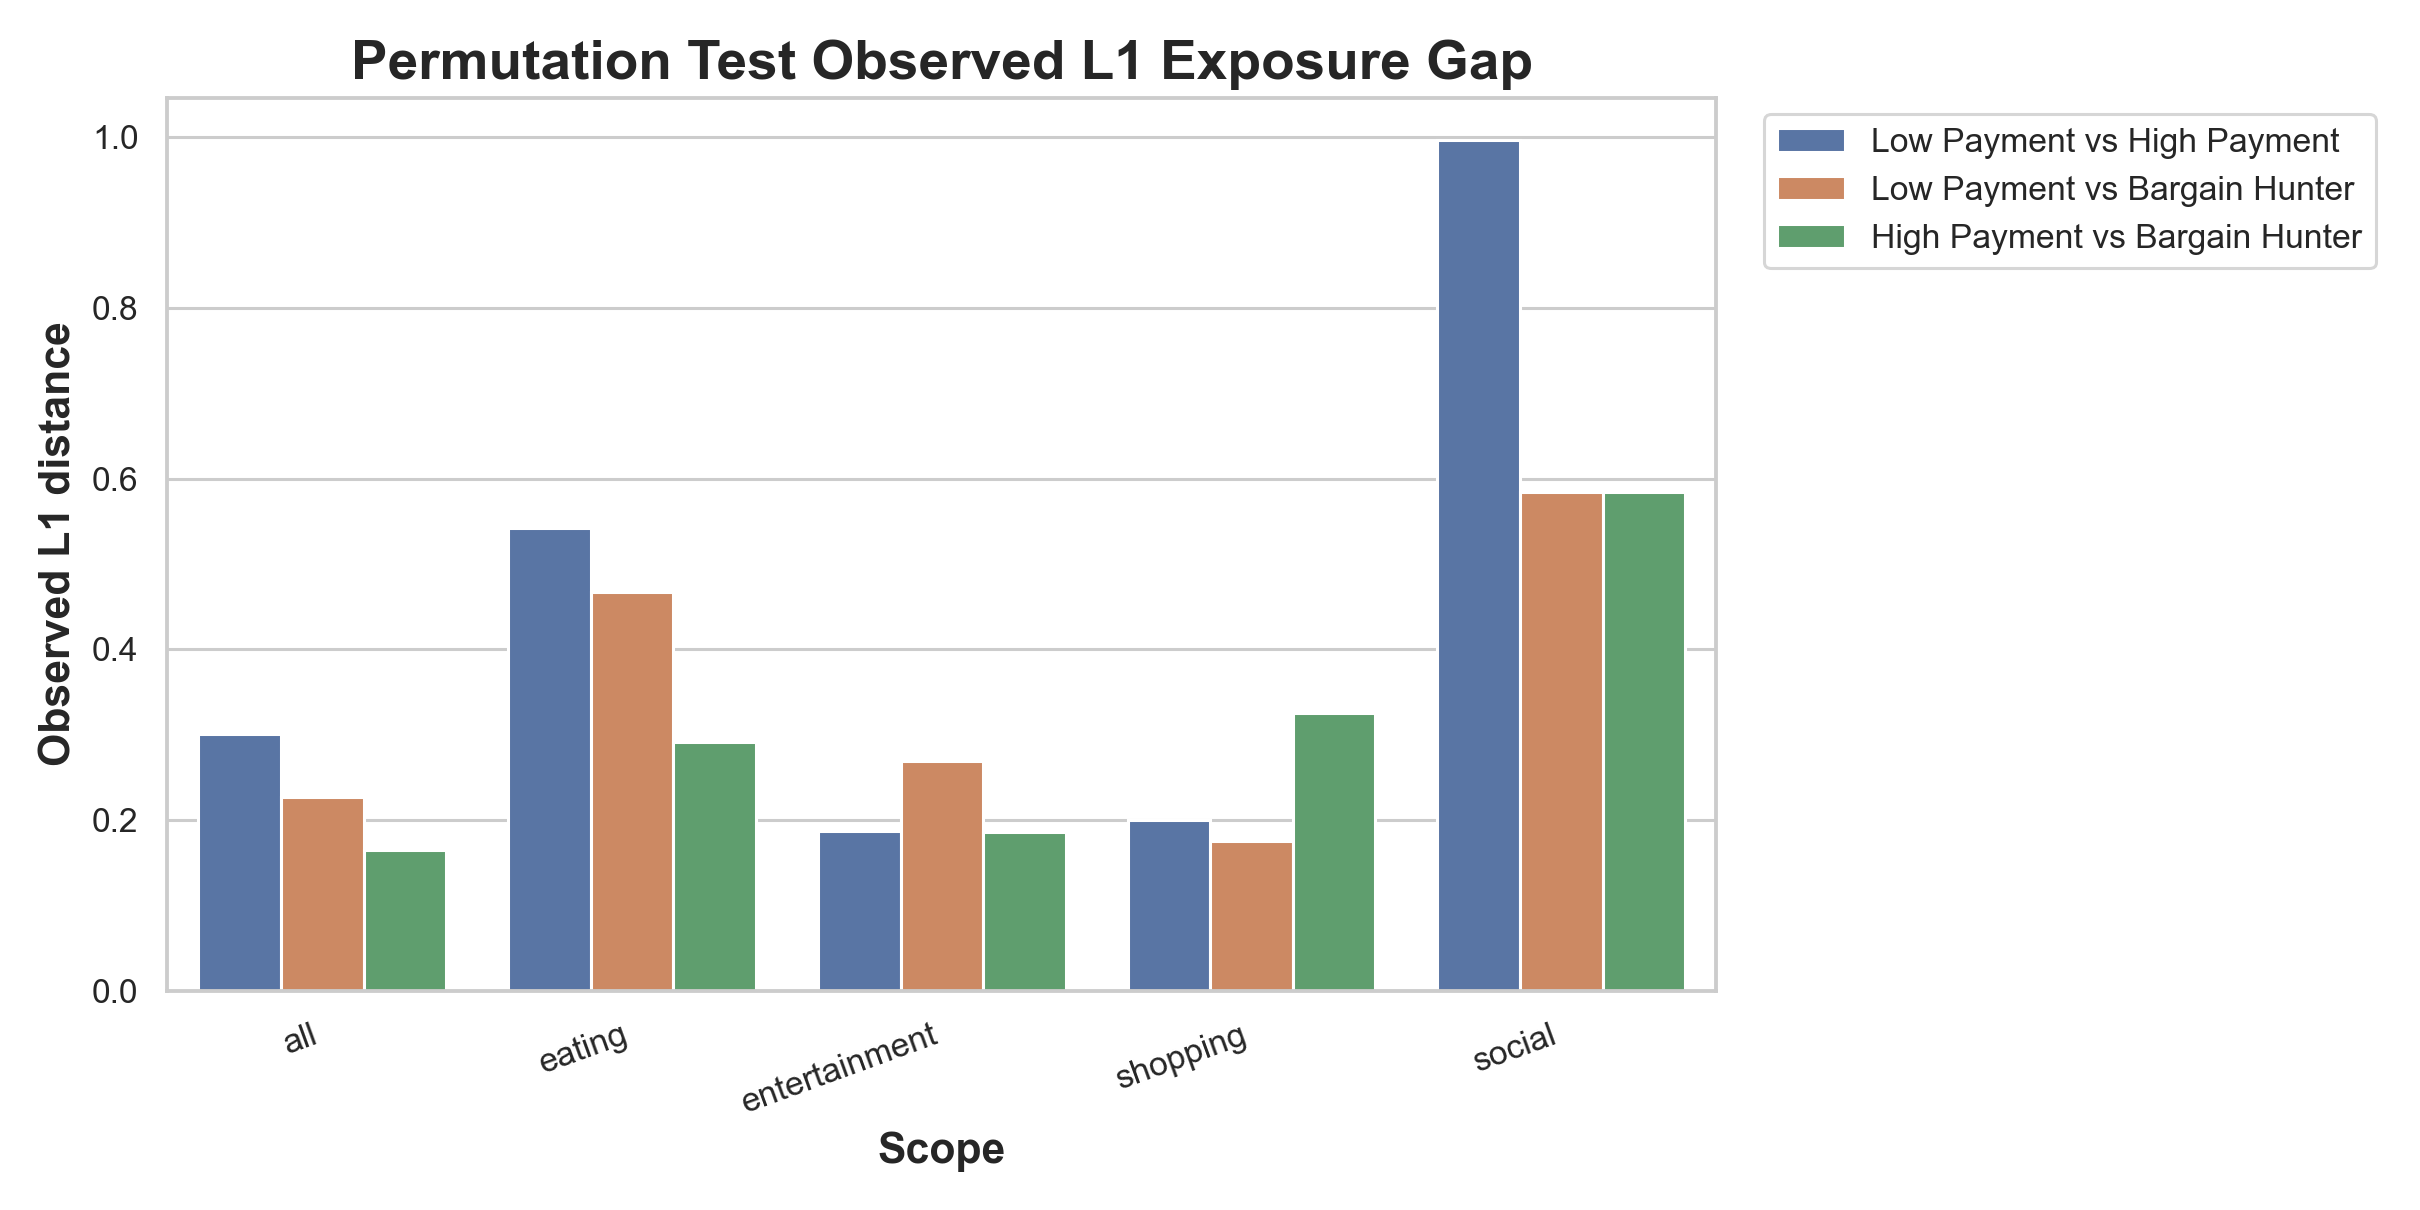
\includegraphics[width=0.95\linewidth]{figures/statistics/permutation_observed_l1_by_scope.png}
    \caption{Representative visualization of observed \(L_1\) exposure distances across comparison scopes based on binarized occurrence \(D_i>0\).}
    \label{fig:method-l1-distance}
\end{figure}

\section{Running Mean Stabilization}

Because a single screenshot can be unstable, the project also examines how exposure estimates change over repeated interaction steps. Early steps may fluctuate because the application has not yet accumulated enough interaction signals, because initial screens contain onboarding or login prompts, or because certain dark pattern mechanisms appear only after specific actions. To observe whether the estimates become more stable, the framework computes a running mean:

\[
\bar{D}_t = \frac{1}{t}\sum_{i=1}^{t} D_i.
\]

The running mean \(\bar{D}_t\) represents the estimated exposure vector after the first \(t\) interaction steps. As \(t\) increases, the estimate incorporates more observations and becomes less sensitive to any single screenshot. These curves are used to examine whether the profile-level exposure estimate stabilizes as more steps are added.

This stabilization analysis evaluates the target 30-step audit budget. If exposure estimates continue to fluctuate heavily after many steps, the audit budget may be insufficient. If the running means gradually stabilize, then the final estimate at the effective trajectory length \(n_{\mathrm{app},A}\) becomes more reliable as a summary of the audited trajectory. In this project, the observed stabilization pattern suggests that repeated interaction is necessary and that the target-budget design provides a more robust estimate than single-state inspection. Nevertheless, stabilization should be understood as empirical support for the audit design, not as proof that all possible long-term exposure patterns have been captured.

\section{Statistical Validation}

The statistical validation layer separates two related but distinct questions.
At the dimension level, the project compares observed exposure values between two profiles with the Mann-Whitney U test.
At the trajectory level, the project uses permutation tests to ask whether the observed profile gap is larger than would be expected after random profile-label reassignment.

The recommended statistical workflow is:
\begin{enumerate}
    \item Compute the observed profile gap, either as a dimension-level difference or as an \(L_1\) distance between profile-level exposure vectors.
    \item Shuffle the profile labels while keeping the DPS observations fixed.
    \item Recompute the gap under the shuffled labels to form a null distribution.
    \item Calculate the permutation \(p\)-value by comparing the observed gap with the null distribution.
    \item Apply multiple-comparison correction to obtain the \(q\)-value.
    \item Report \(L_1\) distance and Cramér's \(V\) as effect-size or association measures.
\end{enumerate}

For the \(q\)-value correction, the report uses Benjamini-Hochberg false-discovery-rate control. This choice is appropriate because the analysis evaluates many profile-dimension and profile-scope comparisons, and the goal is to limit the expected proportion of false discoveries among the reported significant results.

The Mann-Whitney U test is used for dimension-level comparison between two profiles, and its \(p\)-values are then adjusted with the same Benjamini-Hochberg procedure to obtain dimension-level \(q\)-values. The permutation test, by contrast, is reserved for profile-label randomization over the profile-level or category-level exposure gap.

The framework also uses Cramér's \(V\) to measure the strength of association between profile type and DPS exposure. In the reported analysis, Cramér's \(V\) is computed from contingency tables built on binarized DPS occurrence, where each raw score is converted to present versus absent using \(D_i>0\) before tabulation. If future work uses richer ordinal or count scales, the current statistic would require collapsing the positive levels into a binary occurrence indicator or replacing Cramér's \(V\) with an ordinal association measure. In the present report, the binary contingency formulation keeps the statistic aligned with occurrence-rate analysis, while raw means are interpreted as intensity.

Together, Mann-Whitney U tests, permutation tests, Benjamini-Hochberg \(q\)-values, \(L_1\) distance, and Cramér's \(V\) provide complementary evidence. The Mann-Whitney U test evaluates dimension-level separation, the permutation test evaluates whether the observed gap exceeds random reassignment, the \(q\)-value reduces the risk of overinterpreting multiple comparisons, the \(L_1\) distance summarizes the practical magnitude of difference between profiles, and Cramér's \(V\) estimates the association strength between profile type and exposure. By combining these measures, the project avoids relying on a single statistic and provides a more cautious assessment of profile-conditioned dark pattern exposure.

Overall, the differential exposure estimation method treats dark pattern exposure as an empirical, profile-conditioned distribution over interaction states. It does not claim to reveal the internal personalization algorithm of any mobile application. Instead, it measures whether controlled profiles, when interacting with the same applications under reproducible conditions, encounter different patterns of observable dark pattern mechanisms. This framing is consistent with black-box auditing approaches in personalization and platform accountability research, where the goal is to compare observable outputs under controlled conditions rather than to make unsupported claims about internal causality \cite{sandvig2014auditing,hannak2013personalization,srba2023youtube}.
